\documentclass[12pt]{report}
\usepackage{WUthesis}
\usepackage[latin1]{inputenc}
\usepackage{amsmath}
\usepackage{amsfonts}
\usepackage{amssymb} 
\usepackage{graphicx}
\usepackage{notoccite} % Prevents refs in Table of Cont, List of Figs, etc. from starting refs counter.



\begin{document}

\title{Fireball Observation and Analysis using the D6 Surveillance Camera}
\author{Gary Locker}
\thesissupervisor{Dr. Jed Rembold}

\maketitle


\newpage

\begin{center}
\textbf{Presentations and publications:}
\end{center}

List all the posters or oral presentations you have given in physics. Examples are your ATEP thesis proposal talk, your senior progress report in the Fall, SSRD in the Spring, and the combined poster symposium with Linfield at the end of the spring semester.

The format should be 

\begin{itemize}
    \item author, \textit{title}, type of presentation, location, date. 
\end{itemize}

For example,
\begin{itemize}
\item M. Kleinert, J. Kleinert, \textit{Should we get another dog?}, oral presentation, Willamette University, Summer 2019
\end{itemize}

\newpage

\begin{acknowledgments}
By the end of the spring semester, when you turn in your completed thesis for grading, you must have the official acknowledgments listed. Those include mostly funding sources (ask your advisor for help). 

In addition, students often like to add personal thanks to family, friends, or professors. You may add those after you have received your grade and before you upload your final thesis to the academic commons. This is \textit{your} acknowledgment, so you may write whatever you want. Just keep in mind that this thesis is available to other students and faculty. 
\end{acknowledgments}

\newpage

\begin{abstract}
    \begin{general}
        You'll work on two different abstracts: A technical abstract, similar to abstracts you may have seen in publications, and an abstract for a general audience (imagine you want to explain your thesis work to your non-physics friend or family members). You'll work with your advisor on both abstracts over the course of the spring semester. [Adding just a dummy reference here \cite{PBrown2002}.]
    \end{general}
    
    \begin{technical}
        Your technical abstract can go here.
    \end{technical}
\end{abstract}

\newpage


\tableofcontents
\listoftables % Remove if you don't have any tables.
\listoffigures

% Make separate .tex files for each chapter, e.g. introduction.tex, apparatus.tex, etc. That'll make trouble shooting a whole lot easier!
\newpage

Chapter 1: 


On June 2, 2016, a bright object could have been observed streaking through the night sky of Arizona, this object caused sonic booms to occur over the area of Phoenix AR, and reports of this bright object were taken from California, Colorado, Texas, Utah, New Mexico, and Nevada.[\cite{palotai2018analysis}] This is not the first nor last time that an object of this nature will occur in the continental United States, with a more extreme version of this event having occurred in Tunguska in 1908\cite{PBrown2002}.

Just what were these objects that can come streaking in with a brilliant magnitude of light? For that, we must look beyond the Earth's atmosphere and into the neighborhood of the solar system. Where, accompanied by the planets and the sun, are many bits of rock and ice swirling around, some creating swarms that we have nicknamed for when they impact the Earth's atmosphere. These bits of dust and rock are termed either asteroids or meteoroids, depending on their size, as seen in figure 1. 

The concern of this paper however, is on the meteoroids that end up colliding with the Earth's atmosphere, termed meteors, which when impacted the atmosphere, begin to ablate, or burn up, on collision with the air molecules. Without this sphere of atmosphere of course, all of those meteoroids would impact the ground directly, which would be rather catastrophic to human society as a whole. As it is, the ablation of the meteor due to friction from the air molecules causes it to ignite, releasing light and heat into the atmosphere, which is what is observed from the ground.

To capture images of these fireballs, there are many different kinds of camera setups that will be discussed in more detail further into the paper, for now, our attention will be turned to the Willamette D6 AllSky Cam-
era, which operates rather differently from most mainstream methods of fireball detection. Being the size and shape of a short parking bollard, it can easily be picked up and moved to whichever location is deemed to best fit the needs of detection. An added bonus being that there is no super computer involved, just a small microprocessor that uses the camera to view the night sky, only taking captures when the parameters for fireball occurrences are met so as to save space as well as save time when perusing through and analysing the data.

The data being collected can include how long the fireball is observed, the level of brightness it lets off, and other factors, the energy of the fireball can be calculated, known as the optical energy. Peter Brown is an astronomer who found a link between the optical energy of a fireball and the flux, which is an estimate of the density of a given fireball with a certain optical energy. Or in other terms, given the optical energy of a fireball, and using Peter Browns method, it can be determined how many of that type of fireball will collide with the Earth's atmosphere in a given year.

This project will be focused around investigating if the Willamette D6 AllSky Camera, hereby referred to as D6, is an effective alternative for fireball detection, this will be done by comparing our fireball energy size to flux graphs with those given by Peter Brown in his paper, such as the one shown in figure 1.2. Comparing our results to those found in figure 1.2 will give us an idea of how close the data being received by D6 is to the data received by more established methods.




\begin{figure}
    \centering
    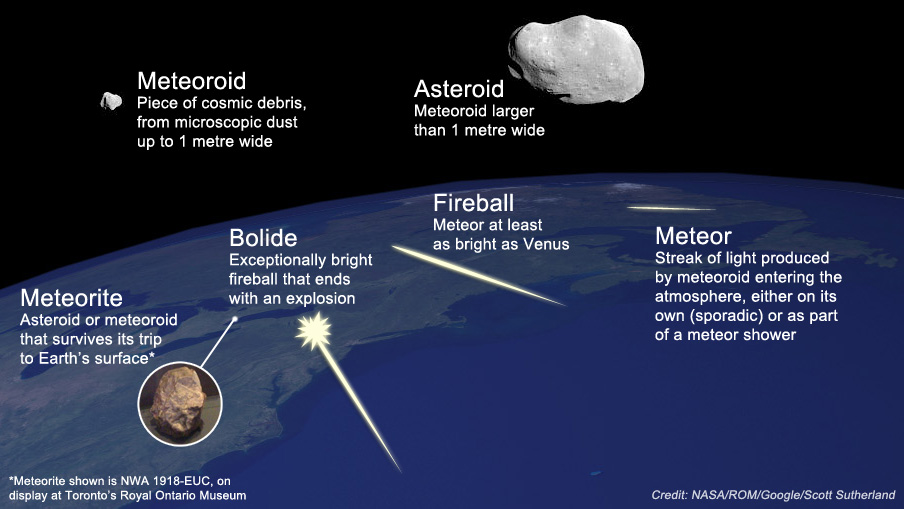
\includegraphics[width=8cm]{Meteor_comparison.png}
    \centering
    \caption{Graphical Overview of the different kinds rock floating around the solar system}
    \label{fig: 1.1}
\end{figure}

\begin{figure}
    \centering
    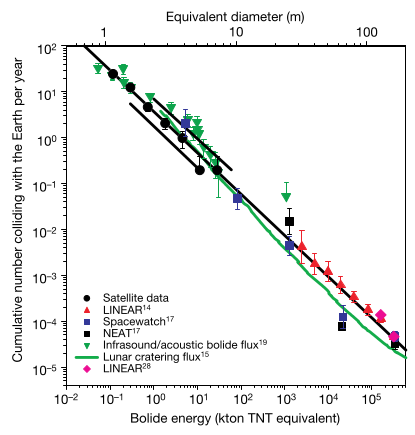
\includegraphics[width=8cm]{flux_brown.png}
    \centering
    \caption{Caption}
    \label{fig: 1.2}
\end{figure}


\newpage

Chapter 2:

(To put into more detail over this week)

Part 1: Talk about fireballs in more depth, discussing how they differ from meteoroids as well as talking about where meteoroids/fireballs come from.

part 2: Types of detection! Focus on systems such as CAMS,SPMN,DFN

part 3: How it's analyzed, discuss Luke's luminosity code, PJ's work with observational area, how we want to measure the flux based off observational energy.

%Chapter 2: 
%\include{apparatus}

%\bibliographystyle{urcsbiblio}
\bibliographystyle{ieeetr}
\bibliography{thesisbib}

\appendix
%\include{notebook}

\end{document}
